\documentclass[12pt,a4paper,utf8x]{report}
\usepackage [frenchb]{babel}
\usepackage[utf8]{inputenc}  
\usepackage[T1]{fontenc} 
% Pour pouvoir utiliser 
\usepackage{ucs}

\usepackage{textcomp}
\usepackage{graphicx}
\usepackage{keystroke}
\usepackage{amssymb}
\usepackage{amsmath}
\usepackage{listings}
%\usepackage{pifont}

\usepackage{url} % Pour avoir de belles url
\usepackage {geometry}
\usepackage[linktocpage]{hyperref}

% Pour mettre du code source
\usepackage {listings}
% Pour pouvoir passer en paysage
\usepackage{lscape}

% Pour pouvoir faire plusieurs colonnes
\usepackage {multicol}
% POur crééer un index
\usepackage{makeidx}
\usepackage{graphicx}
\hypersetup{
backref=true,
%permet d'ajouter des liens dans...
pagebackref=true,%...les bibliographies
hyperindex=true, %ajoute des liens dans les index.
colorlinks=true, %colorise les liens
breaklinks=true, %permet le retour à la ligne dans les liens trop longs
urlcolor= blue, %couleur des hyperliens
linkcolor= blue, %couleur des liens internes
bookmarks=true, %créé des signets pour Acrobat
bookmarksopen=true,
%si les signets Acrobat sont créés,
%les afficher complètement.
pdftitle={Manuel Utilisateur pour LoCD}, %informations apparaissant dans
pdfauthor={MARGUERITE Alain\\ RINCE Romain},
%dans les informations du document
pdfsubject={LoCD}
%sous Acrobat.
}
\makeindex


%%%% debut macro pour enlever le nom chapitre %%%%
\makeatletter
\def\@makechapterhead#1{%
  \vspace*{50\p@}%
  {\parindent \z@ \raggedright \normalfont
    \interlinepenalty\@M
    \ifnum \c@secnumdepth >\m@ne
        \Huge\bfseries \thechapter\quad
    \fi
    \Huge \bfseries #1\par\nobreak
    \vskip 40\p@
  }}

\def\@makeschapterhead#1{%
  \vspace*{50\p@}%
  {\parindent \z@ \raggedright
    \normalfont
    \interlinepenalty\@M
    \Huge \bfseries  #1\par\nobreak
    \vskip 40\p@
  }}
\makeatother
%%%% fin macro %%%%

%Couverture 


\title
{Manuel Utilisateur pour LoCD}



\author{MARGUERITE Alain\\ RINCE Romain}

\date{Université de Nantes \\ 2 rue de la Houssinière, BP92208, F-44322 Nantes cedex 03, FRANCE}

\begin{document}

\maketitle


\clearpage

\tableofcontents
\clearpage

% Pour avoir un interligne de 1,5
\section{Introduction et objectifs}
\label{chap:fichDonnees}
\subsection{Avis au lecteur} 
Ce manuel est destiné à un public désirant utiliser le logiciel GT. C'est à dire depuis son installation jusqu'à la génération du fichier au d'un fichier au format .ktr.Le manuel n'a pas pour objectif d'enseigner l'utilisation de cet outil. Les auteurs recommandes l'ouvrage suivant pour un tel apprentissage : \cite{kiwi}.

\subsection{Présentation du logiciel GT}
GT permet la génération automatique ou manuel de de systèmes temps réel.  L'outil est dédié est uniquement utilisable en mode console.

\section{Installation et configuration}

\subsection{Configuration nécessaire}
\label{sec:conf}
\index{Configuration requise}
\danger : GT est un outil open source dédié uniquement aux systèmes d'exploitation linux. Il n'existe pas encore de version pour Windows et MAC OS. L'installation requière des connaissances dans la manipulation de commandes shell. L'ouvrage suivant est une référence dans ce domaine : \cite{Nutshell}    

\subsection{Installation}
\label{sec:install}
Rendez vous sur \url{http://www.GT.org}. La rubrique «Download» vous proposera une archive de type tar.gz pour différentes distributions (solaris, Linux 32 Bit, Linux 64 Bit, \dots ). Le téléchargement terminé, décompressez l'archive dans le dossier où vous désirez installer GT. Placez vous dans ce dossier et tapez la commande \verb+java -jar GT+. GT est maintenant installé sur votre ordinateur \smiley !!  



\chapter{Utilisation du logiciel grâce à l'interface}\label{chap:usegraph}
  \begin{figure}[htbp]
    \centering
    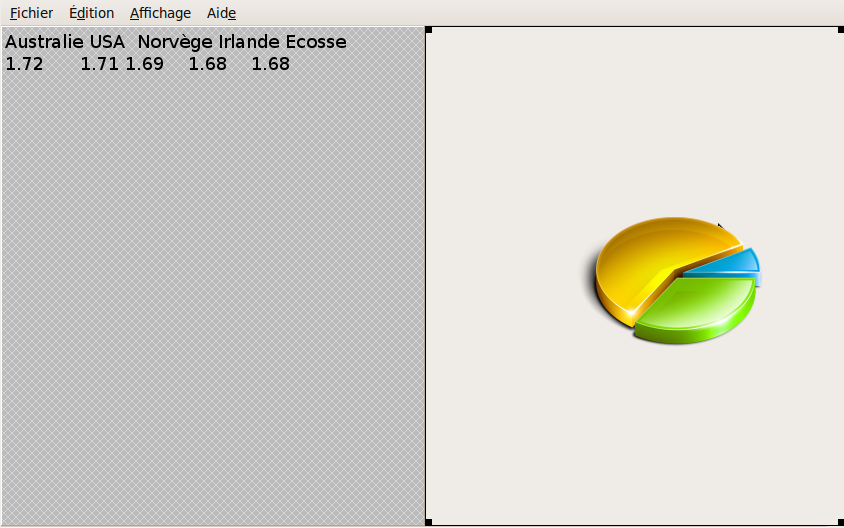
\includegraphics[scale=0.40]{img/soft}
    \caption{Apparence graphique de LoCD}
    \label{fig:apgraph}
  \end{figure}
Pour les utilisateurs peu à l'aise avec l'utilisation des commandes unix, LoCD propose un interface graphique. Bien qu'encore en developpement, cette interface permet de reprendre la plupart des fonctionalités disponibles en lignes de commandes. 
%\clearpage

%%%%%%%%%%%%%%%%%%%%%%%%%%%%%%%%%%%%%%%%%%%%%%%%%%%%%%%%%%%%%%%%%%%%%%%%%

\section{Lancement de l'application graphique}
\label{sec:lancegraph}
Si vous n'avez pas encore installé LoCD sur votre ordinateur, rendez vous à la section \ref{sec:install}. Une fois l'installion complète, il ne reste plus cliquer sur l'executable. Celui ci se trouve à l'emplacement : \verb+/.../LoCD_folder/bin/Locd+. Si un problème à lieu à ce stade, vérifiez que nous avez bien les configurations requises (\ref{sec:conf}). Pour tout autres problèmes \href{mailto:LoCD_assistance@exemple.com}{envoyez nous un mail}.

\section{Utilisation de l'interface graphique}
Voici un bref descriptif des différentes opération proposée par l'interface graphique de LoCD
\subsection{Barre des menus}
Les opérations générales sont listées dans la bare des tâches.
 \paragraph{Fichier}
 \begin{itemize}
\item
Ouvrir : Charger un ficher de données.
\item
Enregistrer : sauvegarder au format «.locd».
\item
Enregistrer sous : préciser le nom de votre sauvegarde.
\item
Exporter : Enregistrer votre diagramme au format de votre choix (pdf ou png).
\item
Quitter : Fermer l'application LoCD.
 \end{itemize} 
 
 \paragraph{Edition}
Ce menu possède le même contenu du menu contextel :
  \begin{figure}[htbp]
    \centering
    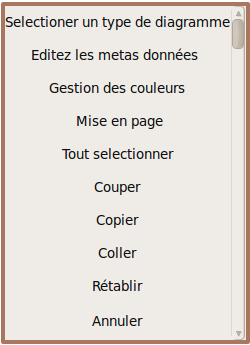
\includegraphics[scale=0.60]{img/menucont}
    \caption{Apparence du menu contextuel}
    \label{fig:menucont}
  \end{figure}

Les opérations : Selectioner un type de diagramme, Editez les metas données, Gestion des couleurs et Mise en page  effectuent les même règlages que ceus décrite dans le chapitre consacré à  l'utilisation par un terminal (\ref{chap:useterm}). Nous vous renvoyons à ce chapitre pour prendre connaissances de ces effets. La seule opération disponible exclusivement dans le menu edition est la rubrique Configuration par défault. Une nouvelle fenêtre s'ouvre et vous propose de régler des différents paramètres (couleurs, mise en page \dots) présents à la figure \ref{fig:dbatons}. 

\chapter{Fichier d'entrée}
\label{chap:fichDonnees}
L'utilisation de LoCD requière en entrée un fichier texte à la sytaxe précise. Ce fichier est composé de deux parties : Méta données et données.
\section{Partie Meta données du fichier d'entrée}
C'est ici que sont définies si besoins les informations décrivant le diagramme. Il est possble d'y préciser 3 sortes d'informations. 
\begin{enumerate}
\item
  Le titre 
\item
  Un sous titre
\item
  Une note
\end{enumerate}
Ces trois donnée doivent être décrite de la manière suivante : 
\begin{enumerate}
\item
  Une ligne par information 
\item
  Une ligne commence par  « > »
\item
  Un des trois mots clefs suivants : \begin{verbatim} TITLE SUBTITLE NOTE \end{verbatim}
\end{enumerate}
Un non respect du format qui va être décrit ci-après soulevera de l'erreur suivante  : 
\begin{figure}[htbp]
  \centering
  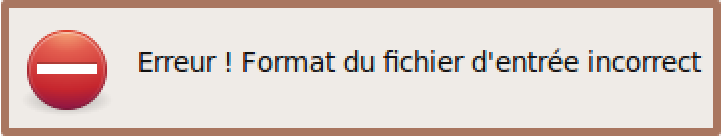
\includegraphics[scale=0.40]{img/eformatfichier}
  \caption{Erreur : format}
  \label{fig:enbdonees}
\end{figure}
Si vous utlisez LoCD avec un terminal, le même texte de l'erreur apparaitra.



\section{Données}
Elles seront renseignées sur deux lignes. La première renseignera les étiquettes des données. Elles seront séparées par un ou des espaces (ou caractères de tabulation). Les valeurs seront sur la ligne suivantes. Les espaces (et\/ou caractères de tabulation) permettent de séparer deux étiquettes ou deux données :
\begin{verbatim}
Etiquette1 Etiquette2     Etiquette3 			Etiquette4
 \end{verbatim} 
 
Toutes les lignes ont une taille d’au maximum 80 colonnes. Dans le cas contraire l'erreur suivante sera relevée : 
\begin{figure}[htbp]
  \centering
  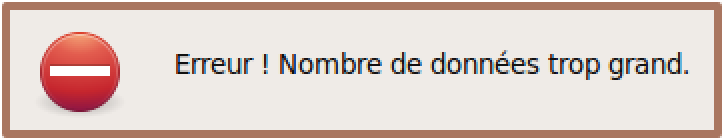
\includegraphics[scale=0.40]{img/enbdonnes}
  \caption{Erreur : nb données}
  \label{fig:enbdonees}
\end{figure}



\section{Exemple de fichier d'entrée}
Pour synthétiser les différents abordés dans ce chapitre voici un exemple de fichier d'entrée valide : 
\begin{verbatim}
  >TITLE: Les plus grands pays du monde pays (~2010)
  >SUBTITLE: En km²
  >Note: La France n'est que 42\up{ème}

  Russie      Canada 	   États-Unis    Chine 	    Brésil 
  17 098 242  9 984 670  9 629 091  	9 596 961  		8 514 877 km2 	
\end{verbatim}
sources \cite{wiki}

\chapter{Fonctionalités}
Nous détaillerons dans cette partie les différentes fonctionalités que propose l'outil. Des exemples illustrés et des \dots  
\section{Histogrammes}
Type de diagramme répendu, l'histogramme fait partie des diagrammes que LoCD peut générer. L'exmple ci-dessus illustre un résultat basique avec la configure par défaut de LoCD soit : 
\begin{itemize}
\item
Une unique couleur : bleu
\item
Absence de titre, sous titre et notes
\item
Représentation 2D
\end{itemize}
Pour changer cette configuration par défault, se référer au chapitre configuration% références !!!!!
\begin{figure}[htbp]
\centering
  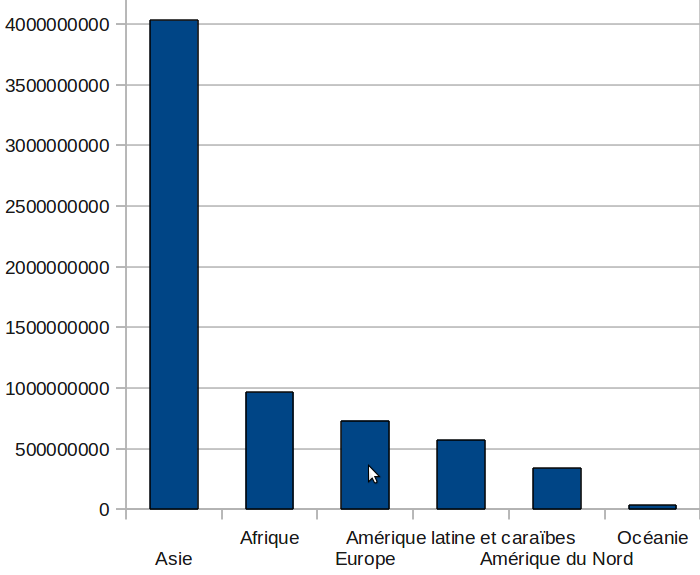
\includegraphics[scale=0.40]{img/diagrammebaton}
  \caption{Histogramme avec les paramètres par défaults}
  \label{fig:dbatons}
\end{figure}
  blah  blah  blah  blah  blah  blah  blah  blah  blah  blah  blah  blah  blah  blah  blah  blah  
\section{Diagrammes circulaires}
LoCD permet la création de diagrammes circulaires similaires  à celui présenté ci-dessous : 
\begin{figure}[htbp]
\centering
  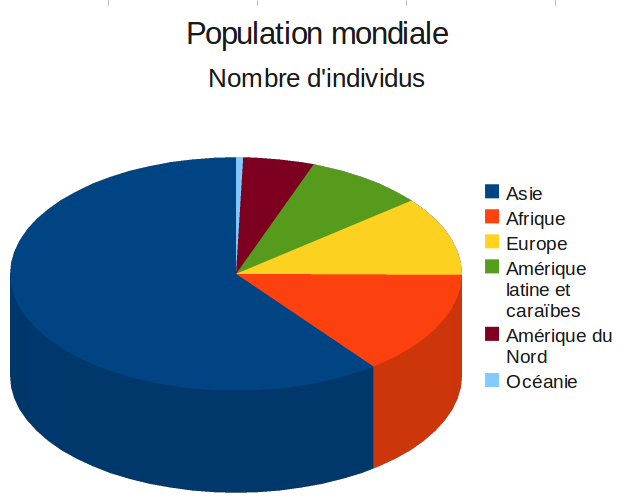
\includegraphics[scale=0.40]{img/diagrammecirculaire}
  \caption{Exemple avec un titre et un sous titre fournis dans les métas données.}
  \label{fig:dcirculaire}
\end{figure}
 blah  blah  blah  blah  blah  blah  blah  blah  blah  blah  blah  blah  blah  blah  blah  blah 
\clearpage
\section{Nuages de points}
\begin{figure}[htbp]
\centering
  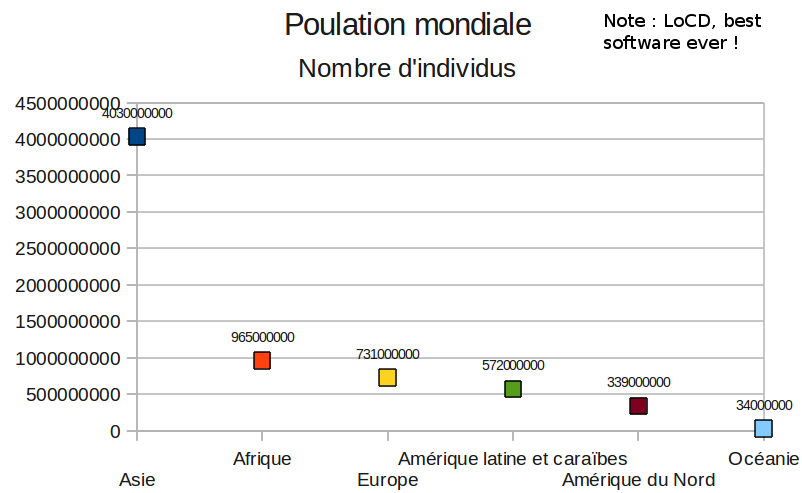
\includegraphics[scale=0.40]{img/diagrammenuages}
  \caption{Nuages de points avec toutes les méta données possible renseignées}
  \label{fig:dnuages}
\end{figure}  
  blah  blah  blah  blah  blah  blah  blah  blah  blah  blah  blah  blah  blah  blah  blah  blah 
  



% Pour finir l'interligne de 1,5

\printindex

\appendix


\end{document}
